
\chapter{Geoestatística utilizando o SGeMS}

O SGeMS (Stanford Geostatistical Modeling Software) é um programa de livre distribuição para a solução de problemas relacionados às variáveis espacialmente relacionadas. Diferentemente dos demais softwares gratuitos, o SGeMS possui interface amigável e de fácil utilização. O software pode ser encontrado no seguinte link \url{http://sgems.sourceforge.net/?q=node/77},  e baixado nas suas respectivas versões 32bits e 64bits. A figura \ref{janela_principal} demonstra a interface principal do programa. 

\FloatBarrier
\begin{figure}[h]
	\centering
	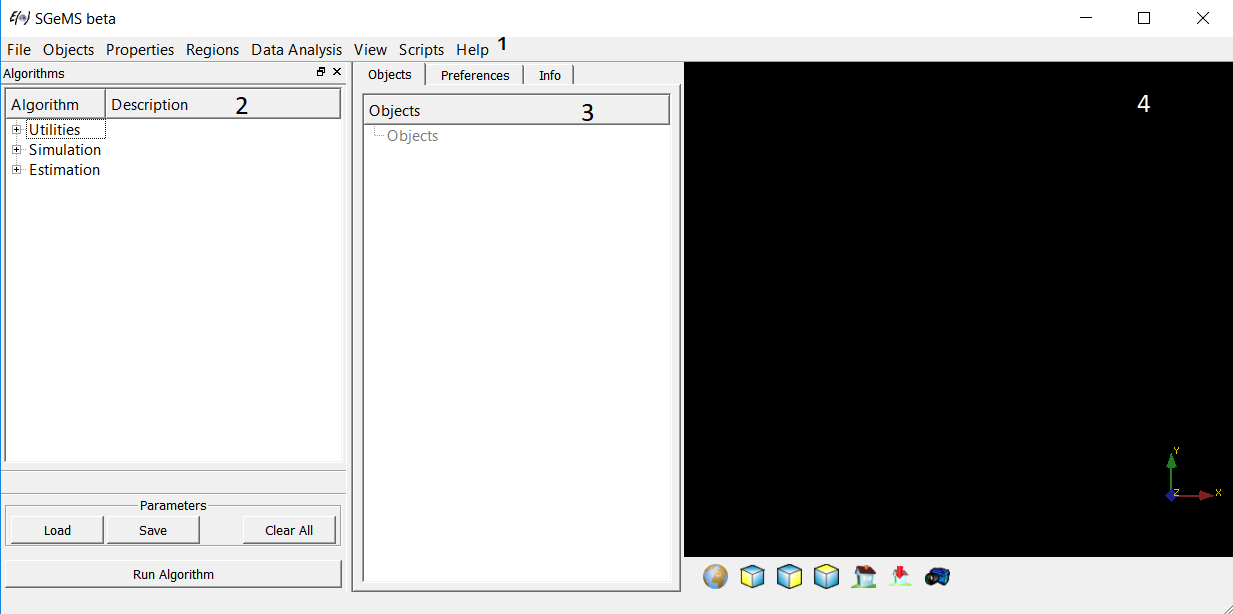
\includegraphics[scale=0.55]{./Capitulo_12/Capturar.png}	
	\caption{ Janela do SGeMs principal. 1) Menu push down contendo principais informações do programa como importação de arquivos, realização de estatísticas e geração de scripts. 2) Aba de algoritmsos contendo os principais algoritmos do SGeMS 3) Objetos importados para o SGeMs como arquivos de pontos ou grids 4) Visualização das informações espacialmente. }
	\label{janela_principal}
\end{figure}
\FloatBarrier

\section{Importando um arquivo de pontos no SGeMS}

Para importar um arquivo de pontos no SGeMs precisamos recorrer ao menu pull down na aba objetos, e em seguida clicar em Load Data. Os arquivos de importação para o SGeMs seguem a mesma referência dos arquivos ASCII importados pelo GSLib, contendo inicialmente o nome do arquivo, número de colunas, nome das variáveis e os dados. Mais informações revisar a seção \ref{Arquivos_GSLIB}.  A figura \ref{Carregar objeto} demonstra o procedimento de entrada. 

\FloatBarrier
\begin{figure}[h]
	\centering
	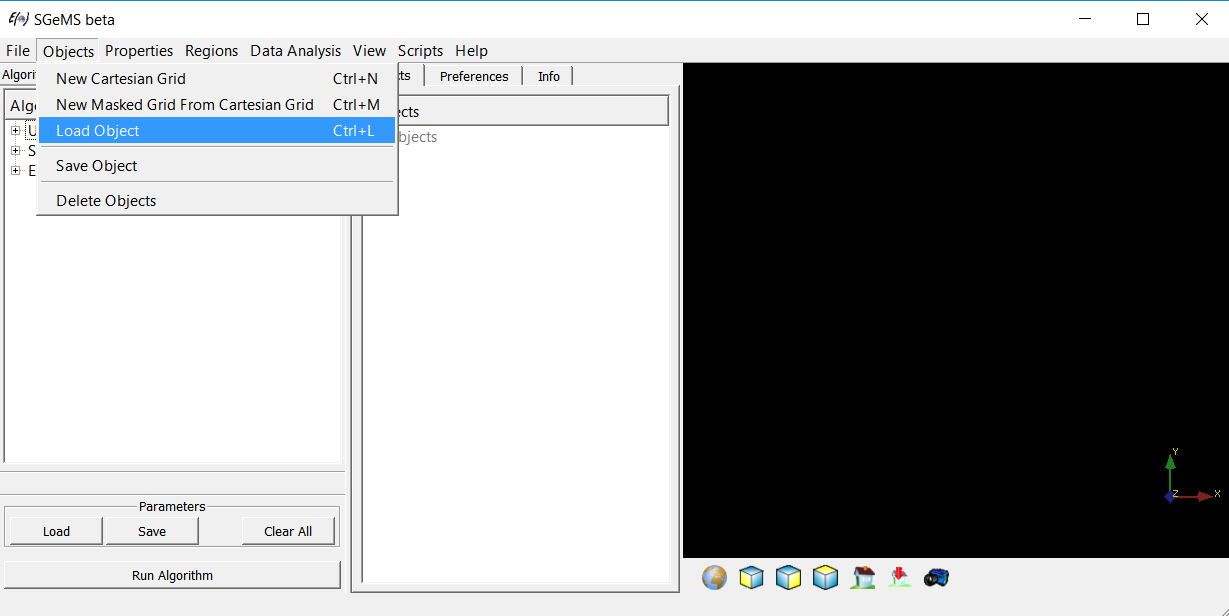
\includegraphics[scale=0.55]{./Capitulo_12/Loadobject.png}	
	\caption{ Importação de arquivo de pontos no SGeMs. Seleção no menu pull down. }
	\label{Carregar objeto}
\end{figure}
\FloatBarrier

Em seguida é aberta uma nova aba para a seleção do arquivo de pontos. Ao escolher o endereço do arquivo é requisitado se o tipo de importação ocorrerá para um arquivo de pontos ou de grid. Neste caso desejamos que o arquivo selecionado seja de pontos. A figura \ref{Carregar objeto_2} demonstra a importação dos dados.


\FloatBarrier
\begin{figure}[h]
	\centering
	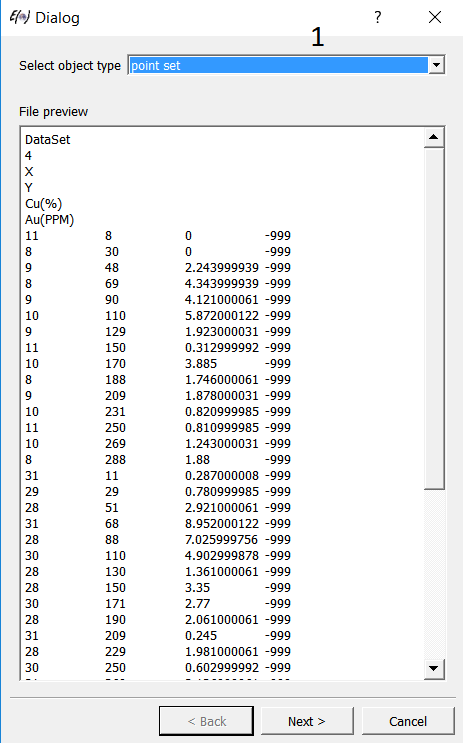
\includegraphics[scale=0.55]{./Capitulo_12/Loadobject2.png}	
	\caption{ Importação de arquivo de pontos no SGeMs. Definição do arquivo de grid. 1) Determinação do arquivo de grids e de pontos.}
	\label{Carregar objeto_2}
\end{figure}
\FloatBarrier

Uma nova aba é aberta possibilitando criar o objeto de pontos no SGeMs. A figura \ref{Carregar objeto_3} demonstra os parâmetros necessários para se criar este arquivo. É necessário atribuir um nome ao objeto, definir quais variáveis são caracterizadas pelas coordenadas espaciais e o número relacionado aos dados faltantes no banco de dados. 

\FloatBarrier
\begin{figure}[h]
	\centering
	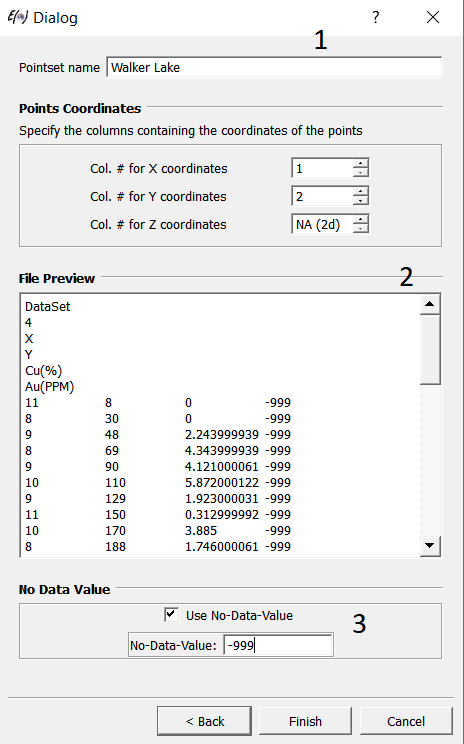
\includegraphics[scale=0.55]{./Capitulo_12/LoadObject_3.png}	
	\caption{ Importação de arquivo de pontos no SGeMs. 1) Denominação do objeto relacionado ao arquivo de pontos no SGeMs 2) Atribuição das variáveis das coordenadas no banco de dados 3) Definição do valor considerado como dado faltante }
	\label{Carregar objeto_3}
\end{figure}
\FloatBarrier

\section{Visualização dos dados - Mapa de localização}

Para visualizar o arquivo de pontos no SGeMs basta selecionar na aba de objetos a propriedade desejada do banco de dados. Ao lado direito, na aba de visualizações, poderá ser observado as amostras com seus respectivos valores coloridos no mapa.

\FloatBarrier
\begin{figure}[h]
	\centering
	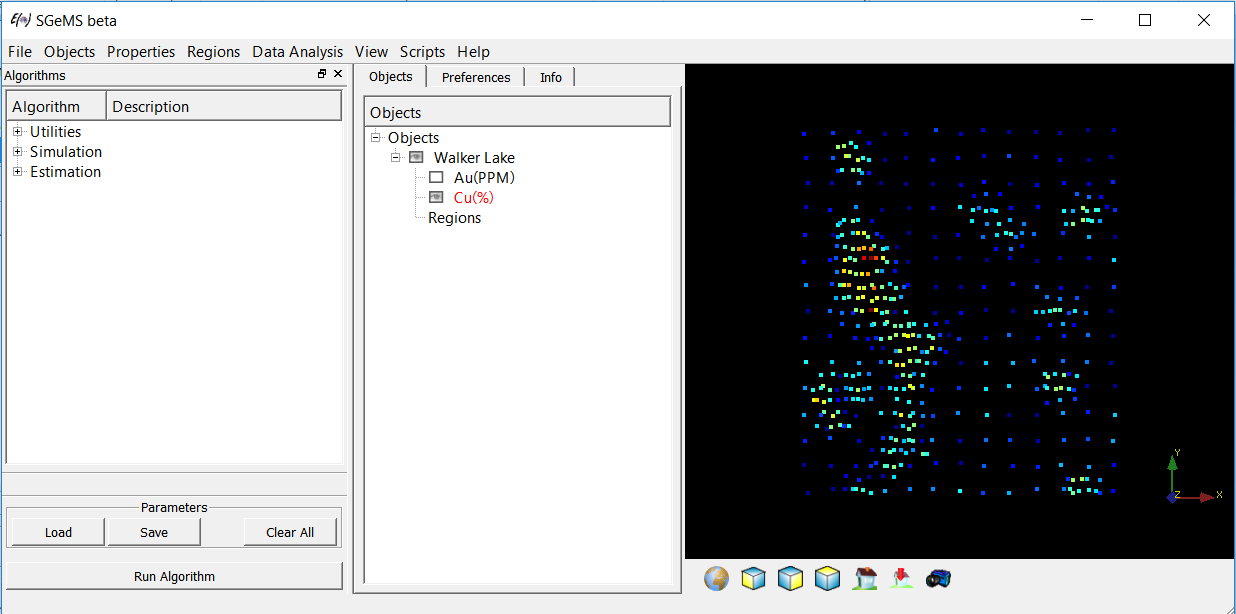
\includegraphics[scale=0.55]{./Capitulo_12/MapLoc.png}	
	\caption{ Mapa de localização da variável Cobre - Seleção da propriedade no menu de objetos }
	\label{Mapa de localizacao}
\end{figure}
\FloatBarrier

\section{Criação do histograma}

Para criar um histograma basta clicar na propriedade considerada com o botão direito e selecionar a opção histograma. A figura \ref{Histograma 1} demonstra os passos necessários para a geração do histograma. 

\FloatBarrier
\begin{figure}[h]
	\centering
	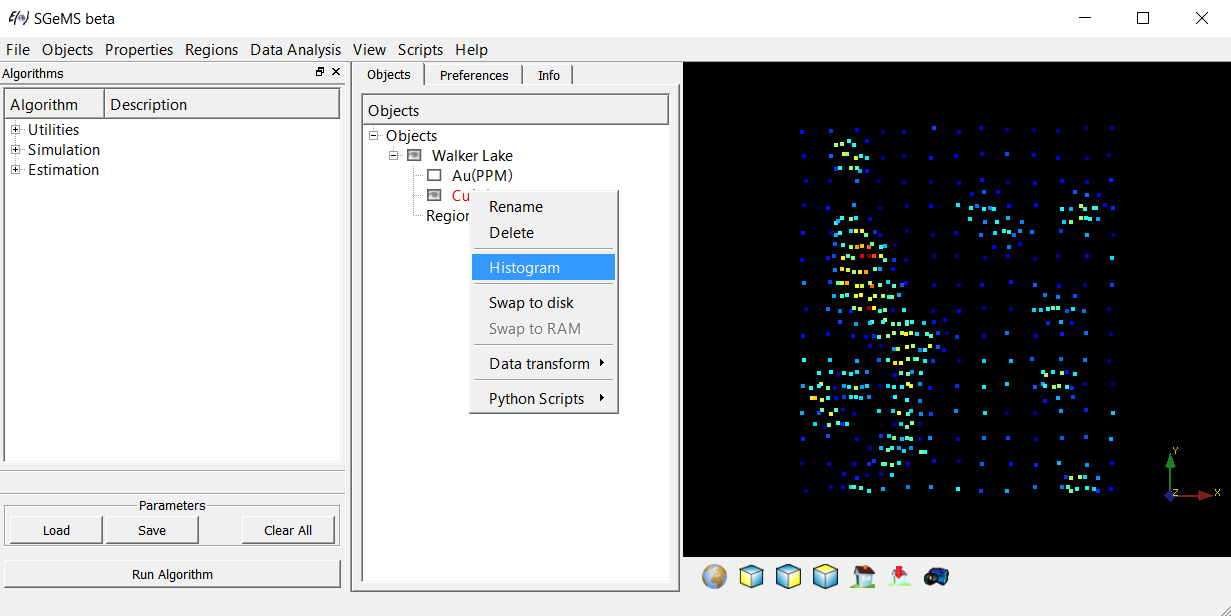
\includegraphics[scale=0.55]{./Capitulo_12/histograma.png}	
	\caption{ Histograma da variável cobre - Seleção pela aba objeto }
	\label{Histograma 1}
\end{figure}
\FloatBarrier

Em seguida é demonstrada a 

\FloatBarrier
\begin{figure}[h]
	\centering
	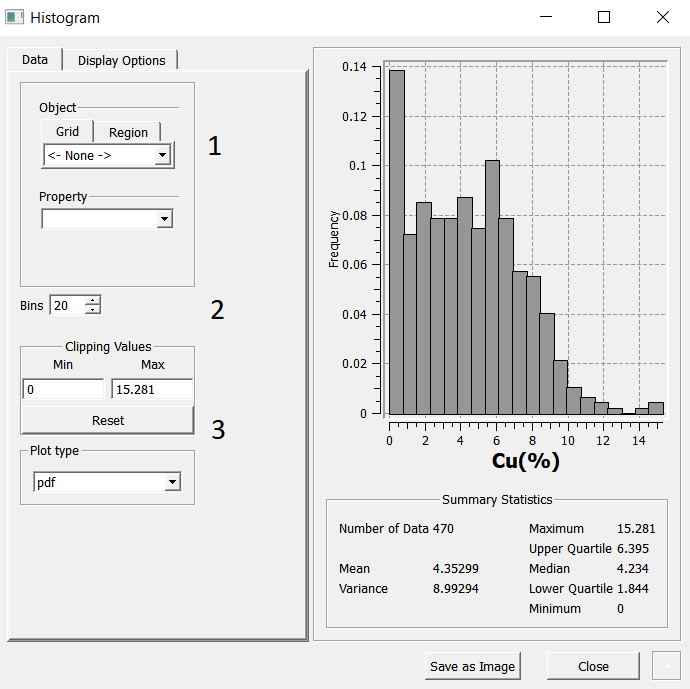
\includegraphics[scale=0.55]{./Capitulo_12/histograma2.png}	
	\caption{ Histograma da variável cobre - Determinação da propriedade e parâmetros. 1) Determinação }
	\label{Histograma 2}
\end{figure}
\FloatBarrier

